\section{实验设计与评价判据}\label{sec:protocol}

\subsection{数据生成过程与双预算制度}\label{sec:dgp}
首先生成平稳高斯 AR(1) 潜过程 $G_t=\rho G_{t-1}+\sqrt{1-\rho^2}\varepsilon_t$，$G_0\sim N(0,1)$，$\varepsilon_t$ 为独立标准正态，$\rho\in\{0,0.8\}$，并舍弃最初 1000 个值。两类观测取
\begin{equation}\label{eq:dgp}
\begin{aligned}
 X_t&=G_t &&\text{（N-AR）},\\
 X_t&=\bigl(\cos2\pi U_t,\ \sin2\pi U_t\bigr)+0.08\eta_t,
 \quad U_t=\Phi(G_t) &&\text{（N-CIRCLE）}.
\end{aligned}
\end{equation}
其中 $\Phi$ 为标准正态分布函数，$\eta_t\overset{\mathrm{iid}}{\sim}N_2(0,I_2)$ 与 $\{\varepsilon_t\}$、$G_0$ 相互独立，$\eta$ 过程与 $G$ 过程独立。$\rho=0$ 时两者均为独立同分布序列，$\rho=0.8$ 时保留较强时间依赖；N-AR 为标量序列（须经时延嵌入），N-CIRCLE 为二维序列（点云直接进入持续同调）。N-CIRCLE 的含噪观测支撑为整个 $\mathbb R^2$，但有限点云在所考察尺度上仍呈明显的环状持续结构。

窗口宽度固定为 $W=64$，步长取 $s\in\{8,16,32,64\}$，对应名义重叠率 $87.5\%$、$75\%$、$50\%$ 与 $0$。两种预算制度为：固定窗口数（fixed-$M$）取 $M=192$，由 $T=W+s(M-1)$ 得 $T=1592,3120,6176,12288$；固定观测长度（fixed-$T$）取 $T=3120$，由式\eqref{eq:windows}得 $M=383,192,96,48$。两者在 $s=16$ 共享 $(T,M)=(3120,192)$，按同一单元计数。每种预算制度含 $2\,(\mathrm{DGP})\times2\,(\rho)\times4\,(s)=16$ 个配置，其中 $s=16$ 的 $4$ 个为共享，去重后共 $28$ 个唯一零假设配置。每格 $2500$ 次主重复、内层 $B=999$，形成 $28\times2\times2=112$ 个“配置—表示—方法”评价单元；主重复在格内相互独立，同一主重复编号在相关条件之间保留配对，内层重采样流与主重复流相互独立。完整窗口几何与乘子带宽见补充材料第~S7.1~节。

\subsection{校准判据与预设主对比}\label{sec:criteria}
记 $\alpha_{\mathrm{eff}}(\theta)=\Pr_{H_0,\theta}\{p_\theta\le0.05\}$，其中 $\theta$ 为数据生成过程、$\rho$、$s$、预算制度、表示与校准方法的组合。逐格报告拒绝率及无连续性修正的 Wilson 区间\cite{Wilson1927}。实用等价带预先取 $\mathcal E=[0.035,0.065]$：$90\%$ Wilson 区间完全含于 $\mathcal E$ 记为实用校准；$95\%$ 区间上界低于 $0.035$ 记为实质保守；下界高于 $0.065$ 记为实质反保守；其余记为未定。该分类是点态判断，不构成设计域上的同时保证。

三项主对比在查看确认性结果前冻结。令 $\pi_{g,\rho,s,m}^{(r)}$ 为 BPI 在预算制度 $r$、校准方法 $m$ 下的零假设拒绝概率，$g\in\{\mathrm{N\text{-}AR},\mathrm{N\text{-}CIRCLE}\}$，则
\begin{equation}\label{eq:primary}
\begin{aligned}
 \mathrm{P1}:\quad D_{\mathrm{OV}}^{M}
 &=\frac12\sum_{g}\Bigl(\pi_{g,0,16,\mathrm{M0}}^{(M)}-\pi_{g,0,64,\mathrm{M0}}^{(M)}\Bigr),\\
 \mathrm{P2}:\quad D_{\mathrm{ST}}^{T}
 &=\frac12\sum_{g}\Bigl(\pi_{g,0,16,\mathrm{M0}}^{(T)}-\pi_{g,0,64,\mathrm{M0}}^{(T)}\Bigr),\\
 \mathrm{P3}:\quad D_{\mathrm{CONS}}
 &=0.05-\frac12\sum_{g}\pi_{g,0,64,\mathrm{M1}}^{(M)} .
\end{aligned}
\end{equation}
P1、P2 检验 $D\le0.10$ 对 $D>0.10$，P3 检验 $D_{\mathrm{CONS}}\le0.01$ 对 $D_{\mathrm{CONS}}>0.01$；两个阈值均为查看结果前规定的最小实质差异，分别对应两 DGP 等权平均下至少 10 个百分点的 I 类错误率差异，以及相对 $0.05$ 至少 1 个百分点的保守偏差。推断使用 10,000 次按数据生成过程分层的整簇自助法：同一主重复编号下的条件、表示与方法随簇共同重采样。单侧 $p$ 值按加一规则计算，边际 $95\%$ 区间取最近秩分位数定义的基本型自助置信区间（basic bootstrap interval），三项 $p$ 值作 Holm 逐步校正\mcite{DavisonHinkley1997,Holm1979}；该区间为边际区间，不解释为 Holm 同时置信区间。MOMENTS 的同构对比仅作次级描述，不进入主要多重性族。完整重采样规格见补充材料第~S3~节。

\subsection{备择构造与尺寸校正功效}\label{sec:alternatives}
以 N-CIRCLE 为基础，在完整序列上连续生成潜变量与噪声，变点取 $\tau=\lfloor T/2\rfloor$，定义
\begin{equation}\label{eq:alternatives}
 X_t=
 \begin{cases}
 C(U_t)+0.08\eta_t, & t\le\tau,\\
 F(U_t)+0.08\eta_t, & t>\tau,
 \end{cases}
 \qquad
 X_t=C(U_t)+0.08\eta_t+0.5\,v\,\mathbf 1\{t>\tau\},
\end{equation}
其中 $C(u)=(\cos2\pi u,\sin2\pi u)$，$F(u)=(\sin2\pi u,\sin4\pi u)$，$v=(\cos2\pi V,\sin2\pi V)$、$V\sim U(0,1)$ 由独立随机流生成并在重复内固定；左式为形状变化，右式为均值平移。当 $U\sim U(0,1)$ 时 $C(U)$ 与 $F(U)$ 的单时点均值均为零、协方差均为 $I_2/2$，加噪后单时点边际矩仍匹配，但完整滞后联合分布未被声明为相同。潜在曲线 $C([0,1])\cong S^1$、$F([0,1])\cong S^1\vee S^1$ 的一阶 Betti 数为 $1$ 与 $2$，然而有限含噪点云的持续图取决于抽样、噪声与尺度，不能保证恰好产生一条与两条长寿命条带。

每个场景取 $M=192$、$s\in\{16,64\}$、$\rho\in\{0,0.8\}$ 共四个条件，每格 $1600$ 次重复。尺寸校正功效使用与备择条件的数据生成过程、依赖水平、窗口几何和表示相匹配的零假设经验临界值：
\begin{equation}\label{eq:power}
 \widehat\beta_{\mathrm{std}}
 =\frac1{R_1}\sum_{r=1}^{R_1}\mathbf 1\bigl\{T_{M,r}^{H_1}>\widehat c_{0.95}^{H_0}\bigr\},
 \qquad
 \widehat c_{0.95}^{H_0}=T_{M,(2376)}^{H_0},
\end{equation}
其中 $R_0=2500$、$R_1=1600$，$2376=\lceil0.95(R_0+1)\rceil$。M0 与 M1 共享同一观测统计量，故每个“条件—表示”组合只计算一次，用于评价表示敏感性，不用于排列两种校准器的优劣。场景层面的表示差 $\Delta$（BPI 减 MOMENTS）由 2000 次联合自助重采样估计。每次分别独立重采样零假设簇与备择簇，BPI 与 MOMENTS 共享对应索引；在四个条件内分别计算功效差，再等权平均形成场景差，区间取最近秩定义的 $2.5\%$ 与 $97.5\%$ 分位数（联合自助重采样规格见补充材料第~S3~节）。

图~\ref{fig:alternatives}展示两类备择的局部点云：图~\ref{fig:alternatives}(a)对应圆形到八字形的变化，图~\ref{fig:alternatives}(b)对应整体平移。示例分别展示 64 个含噪观测点，噪声标准差为 $0.08$；图~\ref{fig:alternatives}(b)取方向 $v=(1,0)$，正式实验中的方向按式\eqref{eq:alternatives}在每次重复内固定。

\begin{figure}[H]
\centering
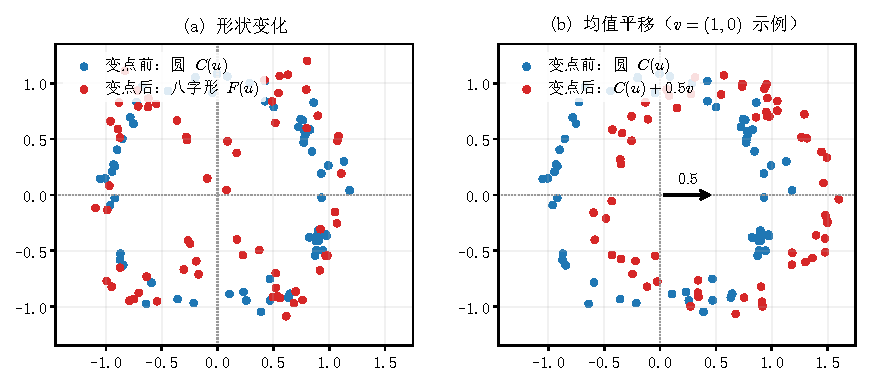
\includegraphics[width=0.90\textwidth]{../artifacts/figures/FigureA_alternative_geometry_short.pdf}
\caption{圆—八字形变化与整体平移备择的点云示意}
\label{fig:alternatives}
\caption*{\footnotesize 注：(a)圆形到八字形；(b)整体平移，示例方向 $v=(1,0)$。}
\end{figure}
